\lettrine{H}{having discussed theories} about how our variables are connected in the in the previous chapter, here I construct a research design for testing the implications of our theory.  It should be remembered that we are trying to answer if a country's linkages to China affects the level of freedom of expression the population enjoys. To achieve this, it is necessary to have access to good quality data and a credible research strategy.

The first part of the chapter features a discussion of the conceptualisation and operationalisation of our two main variables: \textit{linkages} and \textit{freedom of expression}. These are both hard to pin down in a universally accepted manner, which necessitates a thorough explanation of my choices. After discussing the data, the middle part of the chapter will be concerned with the research methodology, specifically how I build the statistical models. This leaves only the end of the chapter; concerning various control-variables which must be incorporated into the model to isolate the actual effect of the linkages from other spurious causes. 

\section{Defining and Operationalising Concepts}
The research question needs a bit more qualification if it is going to be usefully employed. We have two variables main variables, that are more or less broad depending on how they are defined. I treat the specifics in two separate sections below. However, before this I want to include a short treatment of conceptualisation and operationalisation, and why the two are very important steps to include when studying any phenomenon, be they natural or social. 

In the social sciences, defining and operationalising concepts are hard challenges, often harder than in the natural sciences\footnote{It should be noted that even in the natural sciences it can be hard to establish universally agreed upon concepts; nevertheless, the problem is likely far more challenging in social sciences.}, because we most often lack strict separation of the concepts  \citep[for a brief discussion, see:][pp. 360, 392-393]{gerring_what_1999}. An atom is easily differenced from a molecule, but where goes the difference between ideology and belief? There will likely never be complete consensus on every conceptualisation; neither is that necessary. What is most important is that the concepts, from their inception as background concepts, to the eventual scoring of cases is clear and transparent \citep[p. 531]{adcock_measurement_2001}. While we are free to define any concept the way we like, there are some `rules' that should be kept in mind. We should make our concepts familiar, resonant, parsimonious, coherent, differentiated, deep, and useful both in theory and in praxis \citep{gerring_what_1999}. These are all important attributes of a great concept, however, there are always trade-offs between these attributes. As an example, if there is a need to differentiate a concept, this might impair the parsimony of the concept. 

To actually be able to say something interesting I first need to define what I intend my concepts to mean and how far I want them to extend. This is what is known as conceptualisation, and is how we go from a loosely imagined concept to a fully fleshed out one \citep{adcock_measurement_2001, gerring_what_1999}. Here we do not let reality hinder us. The concept should be what we intend it to be, nothing more, nothing less. 

The second phase is where reality comes into the picture. Operationalisation is when we go from the `ideal' concept and translate it to the real world \citep{adcock_measurement_2001}.  From the concept we make indicators, which is how we are able to measure the concept. These indicators are then scored, through the scoring process we are able to gather information about our concept. 

In the next two sections I define the two major concepts used in this study: freedom of expression and linkages. I will do this by utilising a framework of concept development constructed by \citet{adcock_measurement_2001}. Freedom of expression and  linkages are our background concept, and without a more narrow definition, they can mean almost anything.

\section{Dependent variable: \textit{freedom of expression}}
We start by conceptualising and operationalising our dependent variable. There are some challenges when doing this, but the two important points to take from this section is that: one, our definition of freedom of expression is a nuanced one; and two, that this requires us to use a subjective measure of the variable. The operationalisation will be achieved by using the Varieties of Democracy Institute's (V-Dem) Freedom of Expression and Alternative Sources of Information index \citep{coppedge_v-dem_2025}. 

\subsection{Conceptualisation}
Freedom of expression is not at all an easy concept to define in clear terms. Everyone has a basic understanding of the intention: that every person has the right to express their opinion without any obstacles. This is not a wrong perception, but it quickly gets more cloudy when looking at the real world.

Two of the best known definitions are the United Nation's article 19 of the \textit{Universal Declaration of Human Rights} \citeyearpar{un_general_assembly_universal_1948} and the European Union's article 11 of the \textit{Charter of Fundamental Rights of the European Union} \citeyearpar{european_parliament_charter_2012}. The first states that:
\begin{displayquote}
`Everyone has the right to freedom of opinion and expression; this right includes freedom to hold opinions without interference and to seek, receive and impart information and ideas through any media and regardless of frontiers.' \citep{un_general_assembly_universal_1948}
\end{displayquote}
The latter states that:
\begin{displayquote}
`1. Everyone has the right to freedom of expression. This right shall include freedom to hold opinions and to receive and impart information and ideas without interference by public authority and regardless of frontiers.
2. The freedom and pluralism of the media shall be respected.' \citep{european_parliament_charter_2012}
\end{displayquote}
These two are very similar in content, and we can thus read that any definition of freedom of expression should include the possibility of gathering information and imparting information without interference. They also emphasise that access to a pluralistic media environment is important, emphasizing how being able to disseminate information to a wide audience factors into our basic understanding of what freedom of expression should be. This is a good start, but we need to be a bit more clear about what type of expressions we are concerned about and what restrictions are and are not proper when defining freedom of expression. 

I include four important limitations to my conceptualisation of freedom of expression. The first limitation I give freedom of expression in its use here is that it must be a political expression. Thus, we are not moving into the realm of laws against certain types of pornography \citep[pp. 6-7]{bonotti_freedom_2021} or obscene utterances. Many countries have restrictions on certain types of expressions, which they might have a good reason for having. Of course, if the restrictions on non-political expression is used as a tool to silence political expression, they would still qualify as restrictions to political expression.

The second limitation is that the restrictions on freedom of expression must be \textit{de facto} rather than \textit{de jure}. If there are no formal restrictions, but the restrictions of expression still take place, it should count as a restriction of the freedom of expression. On the contrary, if there are legal restrictions, but they are not enforced, e.g., blasphemy laws in western countries, this should not count as a restriction on the freedom of expression. 

The third limitation is that even if the expression is political, restrictions on direct threats and severe forms of libel, should not count negatively for a country's level of freedom of expression. Expressions and actions can in many cases resemble each other, and restrictions on threats and libel to hinder hurt to the object of the expression is not a restriction that imposes itself unduly on the freedom of an actor to expression themself \citep[pp. 81-82]{mill_liberty_2010}. 

The fourth limitation is that certain exceptions should be made. Absolute freedom of expression might on its own be problematic. In the case of Germany there are for instance laws banning expressions of support for Nazism. This is a ban on political expression, however, I would not consider Germany to be repressive because of that. There is context for certain laws, and this should be reflected in the concept, even if we stray from an `ideal.'  

As it stands, our conceptualisation of freedom of expression can be summarised as: \textit{The freedom to express ones'  political opinions, and hear others',  without fear of any repercussions from the state, or other actors, and the content should not be a cause of undue hurt to the object.}

\subsection{Operationalisation}
The above conceptualisation has important implications for how we operationalise freedom of expression. We have many qualifications, and the second limitation forces us not to rely on a simple count of laws limiting freedom of expression, we are better off using a subjective, rather than an objective, assessment of our variable. Subjective variables come with their own challenges, like inter-coder reliability and systematic bias \citep[for a discussion see:][]{little_measuring_2024, miller_how_2024}, however, the gains by using a more nuanced approach makes it a worth while endeavour.

The best and most reliable operationalisation of freedom of expression comes from the V-Dem institute's comprehensive V-Dem dataset \citep{coppedge_v-dem_2025}. The dataset contains many variables and indices used to measure democracy and features relevant to democracy, freedom of expression being a notable one amongst these. The strength of the V-Dem data is that it is thorough, open about its methodology, and includes measures against problems of inter-coder reliability \citep{coppedge_v-dem_2024-2}. (Something about many others using it) There are of course other possible measures to use like Freedom House's \textit{Freedom in the World} dataset \citep{freedom_house_freedom_2024} and the Economist Intelligence Unit's \textit{Democracy Index} \citep{economist_intelligence_unit_democracy_2024}, which both contain variables related to freedom of expression, however, these datasets are hard to disaggregate and have no transparent measures against issues of inter-coder reliability.

Among the variables and indices of the V-Dem dataset we find the Freedom of Expression and Alternative Sources of Information index (henceforth Freedom of Expression index) which we can use as the dependent variable. The variable measures freedom of expression on a theoretical scale from 0 to 1 and answers the question: `\textit{To what extent does government respect press and media freedom, the freedom of ordinary people to discuss political matters at home and in the public sphere, as well as the freedom of academic and cultural expression?}' \citep[pp. 50-51]{coppedge_v-dem_2024-1}. Here 0 denotes a hypothetical country without freedom of expression and 1 denotes a hypothetical country with full freedom of expression. Every real country is somewhere in-between these ideal extremes.

\section{Independent variable: \textit{linkages}}
In this section we define and operationalise our independent variable \textit{linkages}. The linkages are conceptualised as a dyadic relationship between countries in some areas of co-operation. They are further divided into the number of linkages and the size of the linkages. Specifically, I use the Formal Bilateral Influence Capacity index (FBIC) developed and compiled by \citet{moyer_china-us_2021}.

\subsection{Conceptualisation}
Linkages is---in contrast to freedom of expression---relatively easy to define. Not only that, it has been defined for us by the inventors of the concept as used in the field of democratic studies. according to \citet[pp. 383-384]{levitsky_linkage_2006}, linkages can be defined as: `the density of ties and cross-border flows between a particular country and U.S., the EU, and western-dominated multilateral institutions.' \citep[p. 383]{levitsky_linkage_2006} This is a succinct definition, with one glaring problem, I am not interested in links to the West. 

At the most general level, we can define linkages as: \textit{the density of ties and cross-border flows between two countries and their dominant institutions.} This is the most universal conceptualisation of linkages, but for the purposes of this thesis, I can restrict the concept further by including China as the object. This gives us the more differenced concept of linkages.

Thus, linkages to China can be defined as: \textit{the density of ties and cross-border flows between a particular country and China and China-dominated institutions.}

\subsection{Operationalisation}
\citet{levitsky_linkage_2006} also goes a long way to operationalise the concept of linkages, dividing it in five dimensions. The first dimension is economic, the second is geopolitical, the third is social, the fourth is communication related, and the fourth is society related. I would contend that these can be simplified to three main dimensions: economic, geopolitic, and social, as communication and civil society linkages are closely related to the social and geopolitical linkages. 

To each dimension, \citet{levitsky_linkage_2006} includes several indicators, the aggregate of which can go a long way to measure the width and depth of the linkages. The different indicators is summarised in Table \ref{tab:dimensions}. 

\begin{table}[hbt!]
\centering
\caption{Five dimensions of linkages}
\label{tab:dimensions}
\resizebox{\textwidth}{!}{
\begin{tabularx}{\textwidth} {
 >{\noindent\justifying\arraybackslash\hsize=.3\hsize}X 
 >{\noindent\justifying\arraybackslash\hsize=.6\hsize}X
 >{\centering\arraybackslash\hsize=.1\hsize}X}
\toprule
Dimension & Inclusion & FBIC \\
\midrule
Economic linkage
& Trade, investments, credit, and bilateral and multilateral aid flows.
& \checkmark \\
\addlinespace
Geopolitical linkages
& Ties to governments an participations in alliances, treaties, and international organisations
& \checkmark \\
\addlinespace
Social linkages
& Migration, tourism, refugees, diaspora communities, and exchange studies 
& \scalebox{1}[1.5]{$\times$} \\
\addlinespace
Communication linkages
& Cross-border telecommunications, internet connections, and media penetration and coverage 
& \scalebox{1}[1.5]{$\times$} \\
\addlinespace
Transnational civil society linkages
& Local ties to nongovernmental organisations, religious groups, and party organisations
& \scalebox{1}[1.5]{$\times$} \\
\bottomrule
\multicolumn{3}{p{\textwidth}}{\raggedright{\textit{Dimensions are found in \citet[pp. 383-384]{levitsky_linkage_2006}}}}
\end{tabularx}
} % End resizebox
\end{table}

However, there are many linkages, and only some of the data is easily available. I have thus decided to operationalise linkages to China using the Formal Bilateral Influence Capacity index (FBIC), developed by \citet{moyer_china-us_2021}. This is an index that tries to quantify dyadic linkages with a single number. The FBIC index is divided into two parts, bandwidth and dependence, where the former quantifies the extent of the ties and the latter how dependent a country is on another \citep[p. 7]{moyer_china-us_2021}. Dependence is similar to what \citep{levitsky_linkage_2006} terms leverage.

The FBIC index is further divided into three dimensions: economic, security, and political. These correspond most closely to the economic and geopolitical dimensions shown in Table \ref{tab:dimensions} (see column FBIC). The indicators used by Moyer et al. are summarised in Table \ref{tab:fbic} below.

While the FBIC index do lack some of the dimensions and indicators found in \citet{levitsky_linkage_2006}, it is still a good tool for researching the impact linkages have on different countries. Other contributions have already used it to look at how linkages with China might affect media self-censorship \citep{toettoe_foreign_2023}. The main variable of the FBIC is a normalised variable of the weighted variables\footnote{For more information on how the index is calculated, see \citet[pp. 26-31]{moyer_china-us_2021}}, that varies between 0 and 1. 0 means that a country has no influence capacity on another country, and 1 corresponds to the most influence capacity that a country has on another in the dataset \citep[p. 28]{moyer_china-us_2021}. 

\begin{table}[H]
\centering
\caption{Components of the FBIC index}
\label{tab:fbic}
\resizebox{\textwidth}{!}{
\begin{tabularx}{\textwidth} {
 >{\noindent\justifying\arraybackslash\hsize=.15\hsize}X 
 >{\noindent\justifying\arraybackslash\hsize=.425\hsize}X
 >{\noindent\justifying\arraybackslash\hsize=.425\hsize}X}
\toprule
Dimension & Bandwidth & Dependence \\
\midrule
Economic
& Total goods trade & Goods trade, \% of total \\
& Trade agreements & Goods trade, \% of GDP \\
& & Aid, \% of total aid \\
& & Aid, \% of GDP \\
\\
Security
& Total arms transfers & Arms import stock, \% of total \\
& Military Alliances & Arms import stock, \% of military spending stock \\
\\
Political
& Level of diplomatic representation &  \\
& Shared intergovernmental organisation membership & \\
\bottomrule
\multicolumn{3}{p{\textwidth}}{\raggedright{\textit{Information taken from \citet[p. 7]{moyer_china-us_2021}}}}
\end{tabularx}
} % End resizebox
\end{table}

\section{Control Variables}

Since I am using country and time fixed effects, I have to include control variables that changes over time and country. 

In trying to look for evidence of linkages to China affecting freedom of expression, I have to be careful in isolating the relationship between linkages to China and freedom of expression from any other variables that might make the relationship spurious. The main workhorse in removing undesired effects is the fixed-effects model which I will explain below. However, there are some time-varying effects that should be included to prevent us from making wrong inferences. To that effect I have decided to include five additional variables to hopefully reduce the chance of omitted variable bias \citep[pp. 81-85]{wooldridge_econometric_2010}.

The first control variable I include is a variable that measure the impact of a country's linkage to the West. The whole theory of linkages is developed from a point of view that linkages to Western countries can aid democratisation \citep{levitsky_linkage_2006}. It is not far fetched, then, to think that these linkages may also serve to strengthen freedom of expression. If the Chinese influence indeed proves to be able to affect freedom of expression, if not controlled for, linkages to Western countries might obscure this effect. It is also likely that the level of linkages to Western countries fluctuates over a time frame as large as this one (29 years), and this indicates a need to control for this variable. This variable is the sum of the FBIC-score of all `Western' countries. I define Western countries as any West European country, any country with strong inheritance from a Western European country (like the US) and any democratic and strongly Western aligned country (e.g., Japan). The measure is a continuous variable which varies between 0 and 4.85. 0 means zero influence and 4.85 is the highest recorded influence in the restricted dataset (1994-2023). 

The second variable I control for is another important and time-varying effect, namely Gross Domestic Product (GDP) per capita. GDP per capita have been shown to be important for the development and retaining of Democracy. This might be a mutually re-enforcing effect, however, it has been argued that more well-to-do nations, where few live in real poverty is better able to avoid succumbing to demagoguery \citep[p. 75]{lipset_social_1959}. With a general increase in wealth from the early 1990s, this might obscure the effect of Chinese linkages if not controlled for. The variable is the average GDP per capita measured by the World Bank, the International Monetary Found, and the United Nations Statistics Division (CITE). Since the distribution of GDP per capita is very skewed, I have decided to use the log-transformed variable, after which it is a continuous variable between 4.37 and 11.81. 

The third control variable is natural resource rents. Rents from natural resources might have several possible effects on countries. In the one hand, becoming rich might mean that the citizens of a country demand more rights and participation in society, this is maybe especially likely with a moderate increase in rents (CITE). On the other hand, authoritarian regimes in resource rich countries might be able to keep in power by using the resource rents to bribe or repress the population (CITE). To account for this effect, resource rents should be included, as the level of rents might be highly variable for some countries over time. I use the World Bank's World Development Indicators (WDI) measure of total natural resources rents, which measures natural resource rents in per cent of GDP. This varies between 0 and 88.59. 

(Aid is included in the main independent variable FBIC-score, so maybe I shouldn't include it?) The fourth variable is Official Development Assistance (ODA), more commonly known as aid. Aid is likely to be similar to rents, as it might help the government stay in power as it can mitigate problems caused by bad regimes. (BETTER EXPLANATION IS NEEDED)

The fifth and final variable is regime type. Regime type is added for two main reasons. One is to enquire into our second and third hypothesis (\textit{H\textsubscript{2}} and \textit{H\textsubscript{3}}), to see if there are differences between regime types. The second reason is that regime type is another variable that changes with time. To measure regime type, I use the Regimes of the World variable included in the V-Dem dataset. This is an ordinal variable of four levels between 0 and 3. 0 represents an autocracy, 1 represents an electoral autocracy, 2 represents an electoral democracy, and 3 represents a liberal democracy.

In Table \ref{tab:summary} I have included summary statistics for all my variables. 

\begin{table}[H]
\centering
\caption{Summary statistics}
\label{tab:summary}
\begin{tblr}[         %% tabularray outer open
]                     %% tabularray outer close
{                     %% tabularray inner open
colspec={Q[]Q[]Q[]Q[]Q[]Q[]Q[]Q[]},
column{1}={}{halign=l,},
column{2,3,4,5,6,7,8}={}{halign=r,},
}                     %% tabularray inner close
\toprule
& N & Mean & Median & SD & Min & Max & Density \\ \midrule %% TinyTableHeader
Freedom & 5368 & 0.66 & 0.75 & 0.29 & 0.01 & 0.99 & 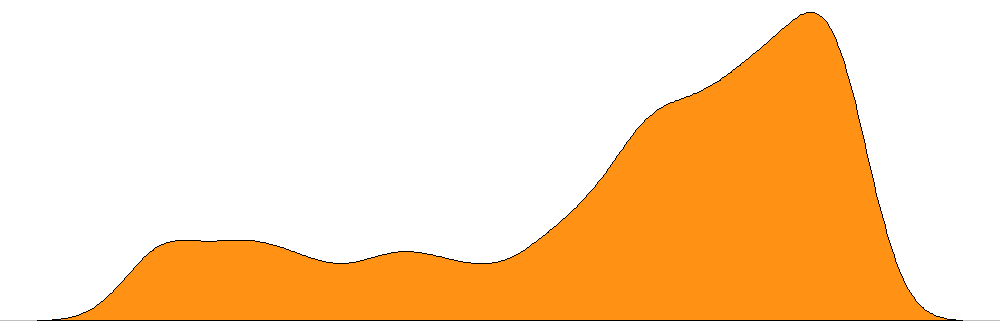
\includegraphics[height=1em]{tinytable_assets/idy1dldkrzo3q9dfcottz3.png} \\
Linkages to China & 5154 & 0.08 & 0.05 & 0.08 & 0.00 & 0.48 & 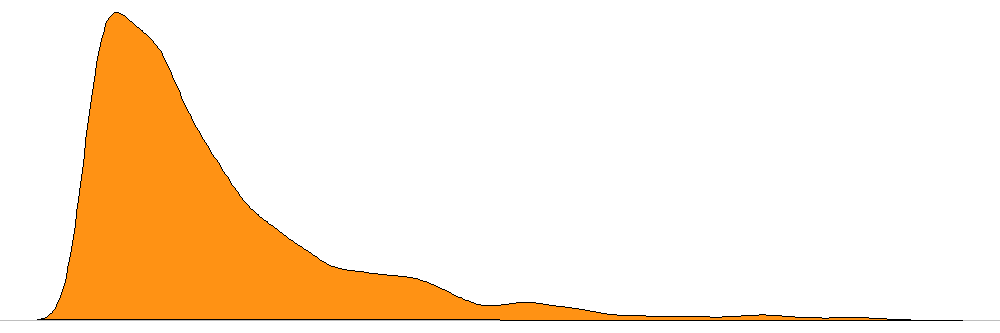
\includegraphics[height=1em]{tinytable_assets/idmgr98k9iwouu5jb9ojjj.png} \\
Regime type & 5368 & 1.59 & 2.00 & 1.00 & 0.00 & 3.00 & 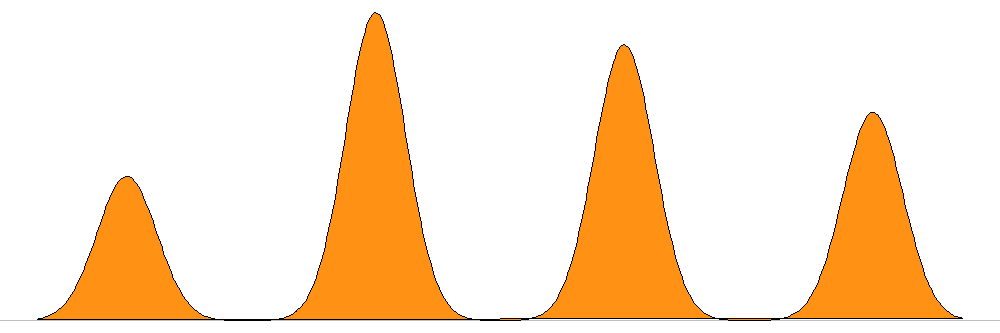
\includegraphics[height=1em]{tinytable_assets/idsc87iypt5fwm3s8gkkyx.png} \\
Linkages to the West & 5154 & 1.08 & 0.68 & 1.08 & 0.03 & 5.32 & 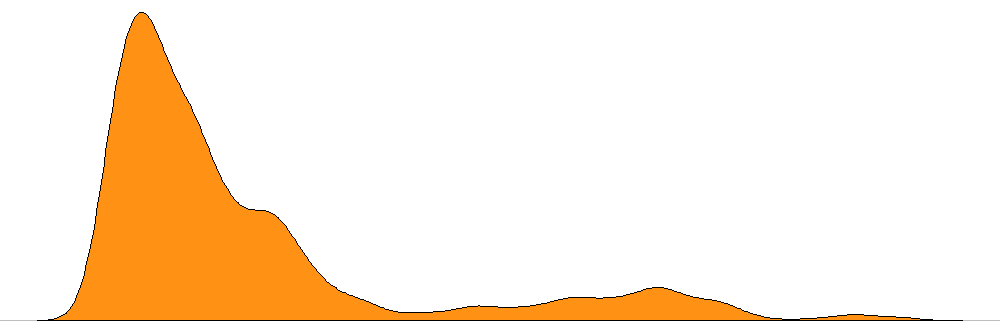
\includegraphics[height=1em]{tinytable_assets/idy3a1puapfh4671ozkrc6.png} \\
GDP per capita & 5190 & 8.20 & 8.16 & 1.58 & 4.37 & 11.81 & 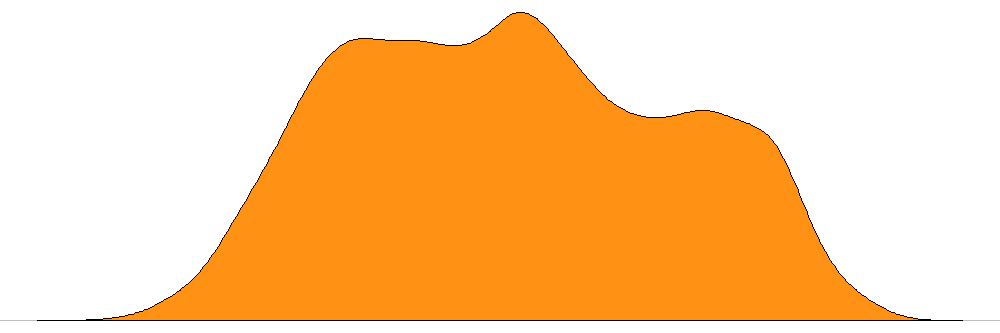
\includegraphics[height=1em]{tinytable_assets/id7rjqfz0gvfsoik7z4rhe.png} \\
Natural resources & 4679 & 7.74 & 2.68 & 11.35 & 0.00 & 88.59 & 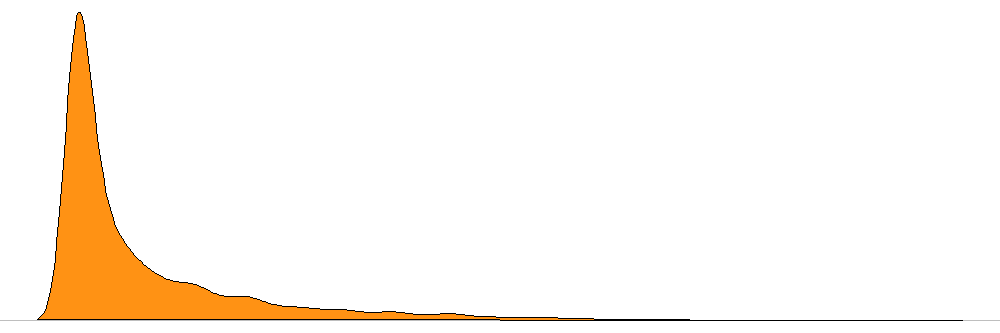
\includegraphics[height=1em]{tinytable_assets/idwq6y16e4psv6gl52yizj.png} \\
Aid & 5213 & 4.25 & 0.78 & 8.01 & 0.00 & 113.13 & 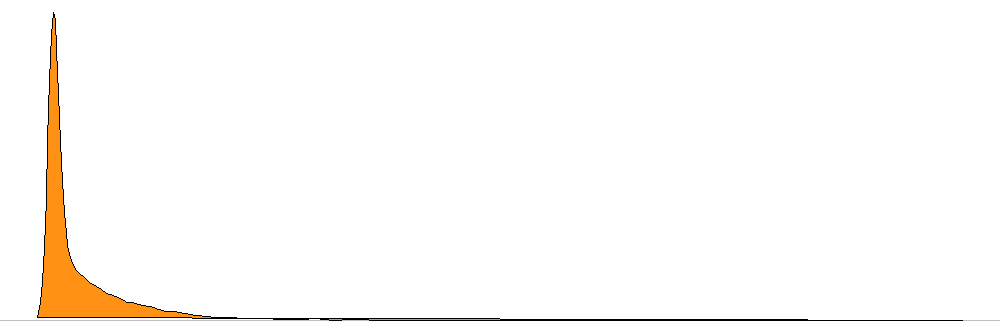
\includegraphics[height=1em]{tinytable_assets/idmsevhk6hz0qvawpig8nj.png} \\
\bottomrule
\end{tblr}
\end{table} 

\section{Observations}
Before diving into the methodology, I would like to summarise the variables and their impact on the research design. First, our unit of analysis---given by our research question---is country-years. I would like to say something about how different countries change over time because of their interaction with other countries. As the data I am using is gathered on the country-level for each year, it means that my unit of observation will be identical to my unit of analysis. Each row in my data is a single country in a single year. Because it is a challenge to define a country, and at what time it came into existence, I include 174 countries where I have data on the two main variables for almost each year from 1994 to 2023. A list of the countries, and as well as the years for which there is data on the variables is included in section \ref{sec:countries} of Appendix \ref{apn:notes}. 

On the one hand, I have the luxury that I do not need to sample my countries, as I have access to data on the whole population I am concerned with. This avoids the problem of sampling bias, which might have occurred if I was forced to choose just some units from a much bigger population. On the other hand, my population (N) is quite restricted as, in the large scheme of things, there are just a limited number of countries. This might be a problem if these countries are very heterogeneous. (MORE on this)

\section{Methodology}
My main objective is to establish if there is---or is not---a negative causal relationship between linkages to China and freedom of expression. To achieve this a sound and transparent methodology is required. In an ideal world, this could have been done by using an experiment, where half the countries would establish linkages with China, and the rest would not. At the same time we would like to hold all other variables constant, so we knew for sure that the changes that were occurring, was caused by the linkages to China.

Alas, this is not possible; next to all countries have extensive linkages to China and there are myriads of variables affecting both freedom of expression and linkages with China. However, this little hypothetical is instructive, as it offers an idealised guide to what needs to be controlled for. E.g., while we cannot have some countries establish linkages and others not, we can look at the difference in linkages, and then how it affects freedom of expression. We also need to know what way the causal mechanism works. Is it the increase in linkages that lead to a decline in freedom of expression, or is it the restrictions put on freedom of expression that is the reason why countries establish ties to China? Maybe people would protest co-operation with China if there was freedom of expression, making it harder to establish ties? I consider it unlikely, specifically because China is too important to the functioning of the international economy. 

\subsection{Variable bias}
We must also recognise that we need to control for three major types of variables. These are variables that are different between units, here the units are countries; variables that are different over time, here the time periods are years; and variables that are different across unit and time, here it would be variables different across country and years. 

The first type of difference to be controlled for, are the differences between countries. Countries can have different regimes, different geographical positions relative to China, and different types of economies, all of which would could have a serious impacts on both on the independent variable of linkages and on the dependent variable that is freedom of expression. E.g., a country could be in a region far away from China with a cultural propensity to value freedom of expression. In this case we would expect the country to have few linkages to China and few restrictions on freedom of expression. These factors, among many, all have to be taken into account when trying to measure the effect of linkages on freedom of expression. 

The second type of difference to be controlled for are time variation. There are many variables that may change over the years; possibly influencing both the dependent and independent variables. One example is economic shocks like the 2008 great economic recession or the corona pandemic, which might have lead to economic linkages around the globe to weaken, and freedom of expression to tumble as regimes try to stay in power in face of public dissatisfaction. Because they affect both of our dependent and independent variables, it is vital for any causal interference that these variables are accounted for when modelling the relationship.

The last type of variation that must be controlled for is variables that changes both between country and years. An example of this is GDP per capita, which differs a lot between countries. In the dataset I use for my models, I examine 174 countries from roughly 1994 to 2023. In 2023 the biggest country difference in GDP per capita was that of Luxembourg and Burundi being almost 129,000 US dollars. The difference is also conspicuous over time, with Luxembourg having the largest difference between its highest and lowest score, at about 90,000 US dollars.\footnote{Note that this number is in current US dollars and is not adjusted for inflation or purchasing power parity. While the actual number would be somewhat smaller, it far outpaces inflation} On the other side of the spectrum we find Burundi, with a maximum difference in GDP per capita just shy of 190 US dollars. Since GDP per capita is both likely to affect how many linkages a country has, with richer countries usually having more linkages and being more open to trade, and freedom of expression, with richer countries usually being more liberal and tolerant of free speech, it is an important variable to account for.

\subsection{Fixed-effects}
There are many challenges to establish a causal link between two variables. Of course, we would in theory like to follow a process in detail at every stage for every unit. This requires resources of a scale that is next to impossible to attain. However, with data on the results and a solid theoretical foundation, it is possible to say something about complex phenomenon. But how is this to be achieved?

I start by calculating the 3 -year difference in FBIC-score. This is done \textit{in lieu} of having access to a treatment and control group with and without linkages to China. In this case we have a pseudo-treatment group with increase in FBIC-score and a pseudo-control group without increase or with decrease. It is important to note that this is nothing  mnemonic; far removed from a laboratory---or indeed a natural experiment. In addition, I lag the dependent variable one year to allow the linkages time to have an effect and to remove any lingering doubt of reversed causality.

To resolve the omitted variable problem, I have decided to use a method called fixed-effects. In very simple terms, fixed-effects is a way to run Ordinary Least Squares (OLS) regression models which accounts for certain effects. These effects must be constant over a certain dimension, e.g., constant for each country or time period. This is achieved by working with the within variation, rather than the absolute variation. This is done by the following procedure (\citeauthor{huntington-klein_effect_2022} \citeyear{huntington-klein_effect_2022}; \citeauthor{wooldridge_econometric_2010} \citeyear{wooldridge_econometric_2010}, pp. 301-302). For all variables we subtract the mean of the time or unit grouped variables from the individual observations. This is described below.

We start with a regular regression model. Here $y$ is the dependent variable, $x$ represent the vector of independent variables, $c$ is the vector of time-invariant factors (note the absence of the subscript $t$), and $u$ is the error term. The subscripts $i$ and $t$ represents the individual unit and time specific observations respectively. We want to remove the $c$ so that it does not effect our error term. 
\begin{equation}
    y_{it} = \beta x_{it} + c_i + u_{it}, \quad i = 1,..., N \quad and \quad  t = 1,..., T  \quad
\label{equ:within_1}
\end{equation} 
We then subtract the mean of the variables:
\begin{equation}
    y_{it} - \bar{y}_i = \beta (x_{it} - \bar{x}_i) + c_i - c_i + u_{it} - \bar{u}_i
\label{equ:within_2}
\end{equation}
leaving us with:
\begin{equation}
    \ddot{y}_{it} = \beta \ddot{x}_{it} + \ddot{u}_{it}, \quad i = 1,..., N \quad and \quad  t = 1,..., T  \quad 
\label{equ:within_3}
\end{equation}
We do the same for time as well, however doing them together is a more complicated process and I use an R-package called \textit{fixest} \citep{berge_efficient_2018} to achieve this. This is, however, the basic form of the process, where I try to remove any variable that is fixed for the units or time periods.

\subsection{The models}
Fixed effects solves the problem of variables that are fixed over time and country influences the results. The last hurdle is to remove effects caused by variables that varies over both time and units. To do this I include the control variables described above. Including these should remove any spurious effects that might cause bias when estimating the relationship between linkages to China and freedom of expression. The final models is represented in the equations below, where Equation \ref{equ:h1} represent a model regressing the dependent and independent variables directly on each other, and \ref{equ:h1_delta} represents a model where the dependent variable is modelled on change in the independent variable.
\begin{multline} \label{equ:h1}
    freedom_{it+1} = \beta_1  linkages_{it} + \beta_2 log(gdppc)_{it} + \beta_3 rents_{it} + \\\beta_4aid_{it} + \beta_5 west_{it} + \beta_6  factor(regime)_{it} + u_{it}
\end{multline}
\begin{multline} \label{equ:h1_delta}
    freedom_{it+1} = \beta_1 \Delta linkages_{it} + \beta_2 log(gdppc)_{it} + \beta_3rents_{it} + \\\beta_4aid_{it} + \beta_5west_{it} + \beta_6 factor(regime)_{it} + u_{it}
\end{multline}
In Equation \ref{equ:h1} the one year lagged freedom of expression variable is a function of  linkages to China, the log-transformed GDP per capita, rents, aid, linkages to the west, regime type, and an error term. Equation \ref{equ:h1_delta}
is almost the same as Equation \ref{equ:h1}, however, the variable for linkages to China now measures the rolling three-year difference in FBIC-score. 

When working with hypotheses two and three, we need a slightly different models from the two above. Instead of including the regime variable as an independent term, we furnish the models with an interaction term between the linkage variable and the factorised regime variable. This makes it possible to see the effect of linkages on different regime types. The interaction models are shown in Equations \ref{equ:h2} and \ref{equ:h2_delta}:
\begin{multline} \label{equ:h2}
    freedom_{it+1} = \beta_1 linkages_{it} + \beta_2 factor(regime)_{it} + \beta_2 log(gdppc)_{it} + \\ \beta_3 rents_{it} + \beta_4 aid_{it} + \beta_5 west_{it} + \beta_6 (linkages * factor(regime)) + u_{it}
\end{multline}
\begin{multline} \label{equ:h2_delta}
    freedom_{it+1} = \beta_1 \Delta linkages_{it} + \beta_2 factor(regime)_{it} + \beta_2 log(gdppc)_{it} + \\ \beta_3 rents_{it} + \beta_4 aid_{it} + \beta_5 west_{it} + \beta_6 (\Delta linkages * factor(regime)) + u_{it}
\end{multline}